\taughtsession{Lecture}{Networking Services: DNS, DHCP, etc}{2023-09-25}{09:00}{Thanos}{}

\textit{Follow up material for lectures will be posted on Moodle. This will commonly include LinkedIn Learning courses. Do them. Answers to Lab Sessions should be uploaded to our individual Wiki sections for each theme as pdf files. They will not be assessed but we may be asked to show them to Lab staff at some point.}

\section{Dynamic Host Configuration Protocol}
\textit{Dynamic Host Configuration Protocol (DHCP)} provides a set of important configuration parameters for devices which are connected to a network. These parameters include: IP address (this is required for any device to be able to talk on a network); router address (the address of the device which your communications has to go through to be passed onto the right place); subnet mask; and DNS server address.\nl

DHCP was introduced in 1993, before DHCP - IP addresses were manually assigned to each device on the network. Whilst, this was a viable option and can still be done to this day - it makes network administrators lives much more complicated. There was also the Bootstrap Protocol (BOOTP) as DHCP supports temporary leases of IP addresses to clients with minimal human interaction. DHCP servers are compatible with BOOTP clients.\nl

For DHCP to work on a network, you require a DHCP server. This commonly is built into modern domestic routers however in larger organisations - a separate (virtual) server will be used.\\

When a client is shut down or it terminates its connection to the internet - it releases it's IP address. This IP address is returned to the IP pool which means it is then available for another client to use. IP address leases are automatically renewed when 50\% of the lease time is used. This works by a request to the original DHCP server. If its not available then the request is broadcast to all available DHCP servers. The IP address lease gets renewed as it prevents the need for a new IP address to be assigned.\\

We use DHCP for a number of reasons: it saves the network administrator from a lot of manual configuration; it allows devices to move from one network to another and gain instant connectivity (there may be conflicting devices if static IPs were used); it allows for more efficient utilisation of available IP addresses (whereby inactive clients do not obtain IP addresses).\\

There are, however, a number of disadvantages to using DHCP: DHCP packets are UDP packets which means they are unreliable and insecure; there is a potential for unauthorised clients obtaining IP addresses which would then make them appear legitimate (this can be avoided by using MAC address filtering); and there is potential for malicious DHCP clients and server which could lead to incorrect configuration parameters being supplied to clients and / or the IP pool being exhausted.\\

\begin{figure}[h]
    \centering
    \includesvg[width=0.9\textwidth]{assets/dhcp-initial-message-flow.svg}
    \caption{DHCP Initial Message Flow}
\end{figure}

\subsection{Terminology}
\begin{description}
    \item[DHCP Packet] DHCP Message
    \item[DHCP Client] Client
    \item[DHCP Server] Server
    \item[Lease] Length of time a DHCP client can use a specified IP address
\end{description}

\section{Domain Name System}
\textit{Domain Name System (DNS)} is the mechanism by which Internet Software translates names to attributes such as IP addresses. Architecturally, DNS is a globally distributed, scalable and reliable database which is comprised of three components: a \textit{namespace}, \textit{servers} (makes the namespace available) and \textit{resolvers} (clients - these query the servers about the namespace).\\

DNS exists to make users' use of the internet easier. Users generally prefer names (\verb|thomasboxall.net|) to numbers however computers usually prefer numbers (\verb|145.14.152.146|) to names. DNS provides the mapping between the \textit{domain names} and \textit{IP addresses of servers}. \\

DNS is distributed globally throughout many different devices. No single computer holds all the DNS data, however some remote DNS data is locally cached to improve performance. DNS lookups can be performed by any device. DNS lookups can be performed by any device. On UNIX systems, the command \verb|dig| provides this utility.\\

The DNS database is always internally consistent. This is achieved by each version of a subset of the database (a zone) having a serial number which is incremented on every database change. Changes to the master copy of the database are replicated according to timing set by the zone administrator, generally this is quite frequent. Cached data expires according to a timeout set by a zone administrator. While there is no limit to the size of the DNS database, common sense dictates that its not a  good idea to store 200,000,000 domain names in the same database as there is no limit to the number of queries. This can lead to 10,000+ queries being sent each second which are handled easily. Queries are distributed among primary and secondary DNS servers as well as caches. The \verb|nslookup| command will tell you where it has obtained the DNS information from.\\

Due to DNS data being replicated from the primary to multiple secondary servers, there is high levels of reliability. Clients will typically query local caches first, and if they do not contain the data requested then the queries will be passed to either the primary server or any secondary server. DNS uses both UDP and TCP (port 53) for different things: TCP is used for intra-server communications and UDP is used for communications between clients and servers.\\

The DNS database can be updated dynamically. This includes the addition, deletion or modification of any record. However, it is only the primary server which can be dynamically updated. The modification of the primary database triggers replication to all the secondary databases.

\section{Domain Names}
A domain name is the sequence of labels from a node to the root, separated by dots (\verb|.|) which is read from left to right. The namespace has a maximum depth of 127 levels and domain names are limited to 255 characters in length. A nodes domain name identifies its position in the namespace.

\begin{figure}[H]
    \centering
    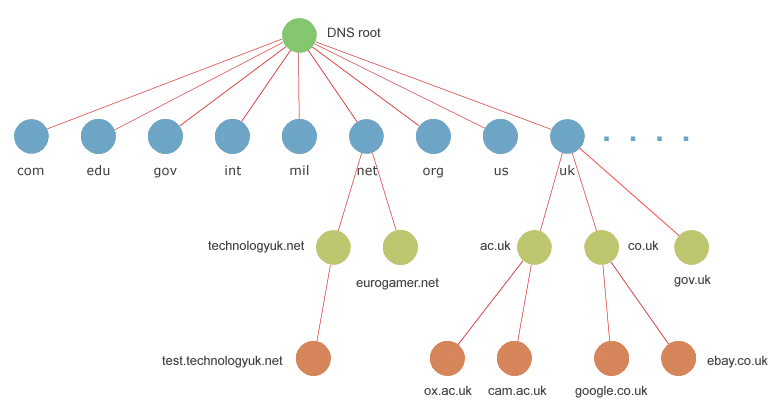
\includegraphics[width=0.8\textwidth]{assets/dns-structure.png}    
    \caption{DNS Structure}
\end{figure}

One domain is a subdomain of another if its domain name ends in the other's domain name. 

\begin{figure}[H]
    \centering
    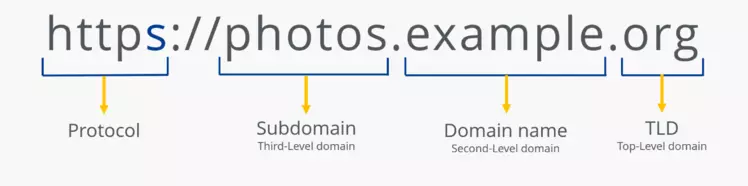
\includegraphics[width=0.9\textwidth]{assets/domain-anatomy.png}    
    \caption{Anatomy of a domain}
\end{figure}

Name servers store information about the namespace in units called \textit{zones}. The nameservers that serve a complete zone are said to \textit{have authority} or \textit{be authoritative for} the zone. More than one name server can be authoritative for the same zone, ensuring redundancy and load spreading. Also, a single name server may be authoritative for many zones. There are two types of Name Servers: \textit{authoritative} which maintains the data (has subtypes of primary and secondary) and \textit{non-authoritative} which caches the authoritative server. No special hardware is needed for a name server.\\

Name resolution is the process by which local resolvers and the nameservers cooperate to find data in the namespace. Upon receiving a query from a resolver, a name server:
\begin{enumerate}
    \item looks for the answer in its authoritative data and its cache.
    \item if step 1 fails, the answer must be looked up through other servers (this can either be done recursively or iteratively).
\end{enumerate}